\label{sec:joining_a_tean}
\begin{figure*}
  %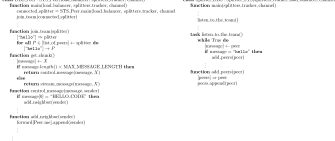
\includegraphics[width=\textwidth]{joining}
  \fig{700}{7cm}{joining} \caption{Procedures run when a peer
    joins a team.\label{fig:joining_a_team}}
\end{figure*}

Incoming peers 

As can be seen in Fig.~\ref{fig:joining}, incoming peers request
(using a reliable communication) to the splitter the current list of
peers in the team. To minimize the joining time, the peer sends a
$[\mathtt{hello}]$ message to each peer of the team in parallel with
the reception of the list. When a peer of the team receives a
$[\mathtt{hello}]$, it runs the $\mathrm{add}\_\mathrm{neighbor}()$
function, which basically: (1) adds the sender of the message to a
table of peers called $\mathrm{forward}[]$ (if in peer $P_i$ there is
an entry $\mathrm{forward}[P_j]=P_k$ then, each chunk received by
$P_i$ and originated at $P_j$ will be forwarded to $P_k$), initializes
the table $\mathrm{debt}[]$ (which stores the chunk debts between
neighbor peers), and (3) sets the variable $\mathrm{neighbor}$ with an
index to $\mathrm{forward}[]$ (see
Sec.~\ref{sec:chunk_DBS_processing}).

The splitter, in an infinite loop: (1) listens to the peers, (2) sends
the list of peers in the team to the peers, (3) adds the incoming peer
to the list, and (4) sends to the teams tracker the number of peers
in the team.
